\documentclass[conference]{IEEEtran}
\usepackage{cite}
\usepackage{amsmath,amssymb,amsfonts}
\usepackage{graphicx}
\usepackage{textcomp}
\usepackage{xcolor}
\usepackage{url}
\usepackage{booktabs}

\begin{document}

\title{Task [B1]: [Detecting Fraudulent Job Postings]}

\author{\IEEEauthorblockN{Muhammad Zaryab Attiq}
\IEEEauthorblockA{Roll No. 70176119 \quad Section A\\
Repository: \url{https://github.com/Muhammad-Zaryab-Attiq/AI101-ML-Assignment-70176119}\\
Instructor: Dr. Muhammad Awais, AI Architect}
}

\maketitle

\section{Introduction}
The rapid proliferation of remote recruitment platforms has intensified online employment fraud, exposing candidates to identity theft and advance-fee wire schemes. In this study, we formulate an imbalanced binary classification framework on the Employment Scam Aegean Dataset (EMSCAD) containing 17,880 postings, where only 4.84\% are fraudulent. By fusing unstructured text fields (descriptions, requirements, benefits) with structured metadata (missingness indicators, company logo presence, telecommuting status) via a zero-leakage scikit-learn \texttt{ColumnTransformer}, our champion multimodal model achieves an $F_1$ score of 0.835 on the fraud class and a PR-AUC of 0.907, outperforming models reliant purely on administrative structured metadata by over 159\% in $F_1$ gain.

\section{Problem Statement}
Given an input tuple $x = (x_{\text{text}}, x_{\text{struct}})$ representing free-text job content alongside categorical and binary administrative metadata, our task is to learn a decision classifier $f: x \mapsto y \in \{0, 1\}$, where $y=1$ denotes a fraudulent advertisement and $y=0$ denotes a legitimate one. Because the dataset exhibits extreme class imbalance (95.16\% negative vs. 4.84\% positive), standard accuracy is uninformative. Success is defined primarily by the Area Under the Precision-Recall Curve (PR-AUC) and the $F_1$ score on the positive (fraud) class, with the decision threshold $\tau$ calibrated on a held-out validation split.

\section{Dataset Used}
We employ the Real or Fake Job Postings dataset (EMSCAD) hosted on Kaggle~\cite{vidros2017}. The corpus comprises 17,880 job advertisements described by 17 features: 5 free-text fields (\texttt{title}, \texttt{company\_profile}, \texttt{description}, \texttt{requirements}, \texttt{benefits}), 6 categorical attributes (\texttt{employment\_type}, \texttt{required\_experience}, \texttt{required\_education}, \texttt{industry}, \texttt{function}, \texttt{location}), and 3 binary indicators (\texttt{telecommuting}, \texttt{has\_company\_logo}, \texttt{has\_questions}). We explicitly engineer missingness indicators for key fields because missing company metadata provides a strong inductive signal of fraud.

\section{Dataset Statistics}
Table~\ref{tab:dataset_stats} provides the summary statistics for the EMSCAD corpus. Text lengths vary substantially between classes: legitimate postings have a higher median word count (248 words) than fraudulent postings (178 words). Furthermore, postings lacking a company logo exhibit an elevated fraud rate of 15.8\%, compared to only 3.1\% for logo-bearing postings.

\begin{table}[htbp]
\caption{Dataset statistics.}
\label{tab:dataset_stats}
\centering
\begin{tabular}{lr}
\toprule
\textbf{Property} & \textbf{Value} \\
\midrule
Samples (after cleaning) & 17,880 \\
Features (numeric / categorical / text) & [2 / 10 / 5] \\
Target classes & Binary (0: Real, 1: Fraud) \\
Class distribution & 17,014 Real / 866 Fraud (4.84\%) \\
Missing values (company profile / salary) & 18.50\% / 83.96\% \\
Train / validation / test split & [12,516 / 2,682 / 2,682] (70 / 15 / 15) \\
\bottomrule
\end{tabular}
\end{table}

\begin{figure}[htbp]
\centering
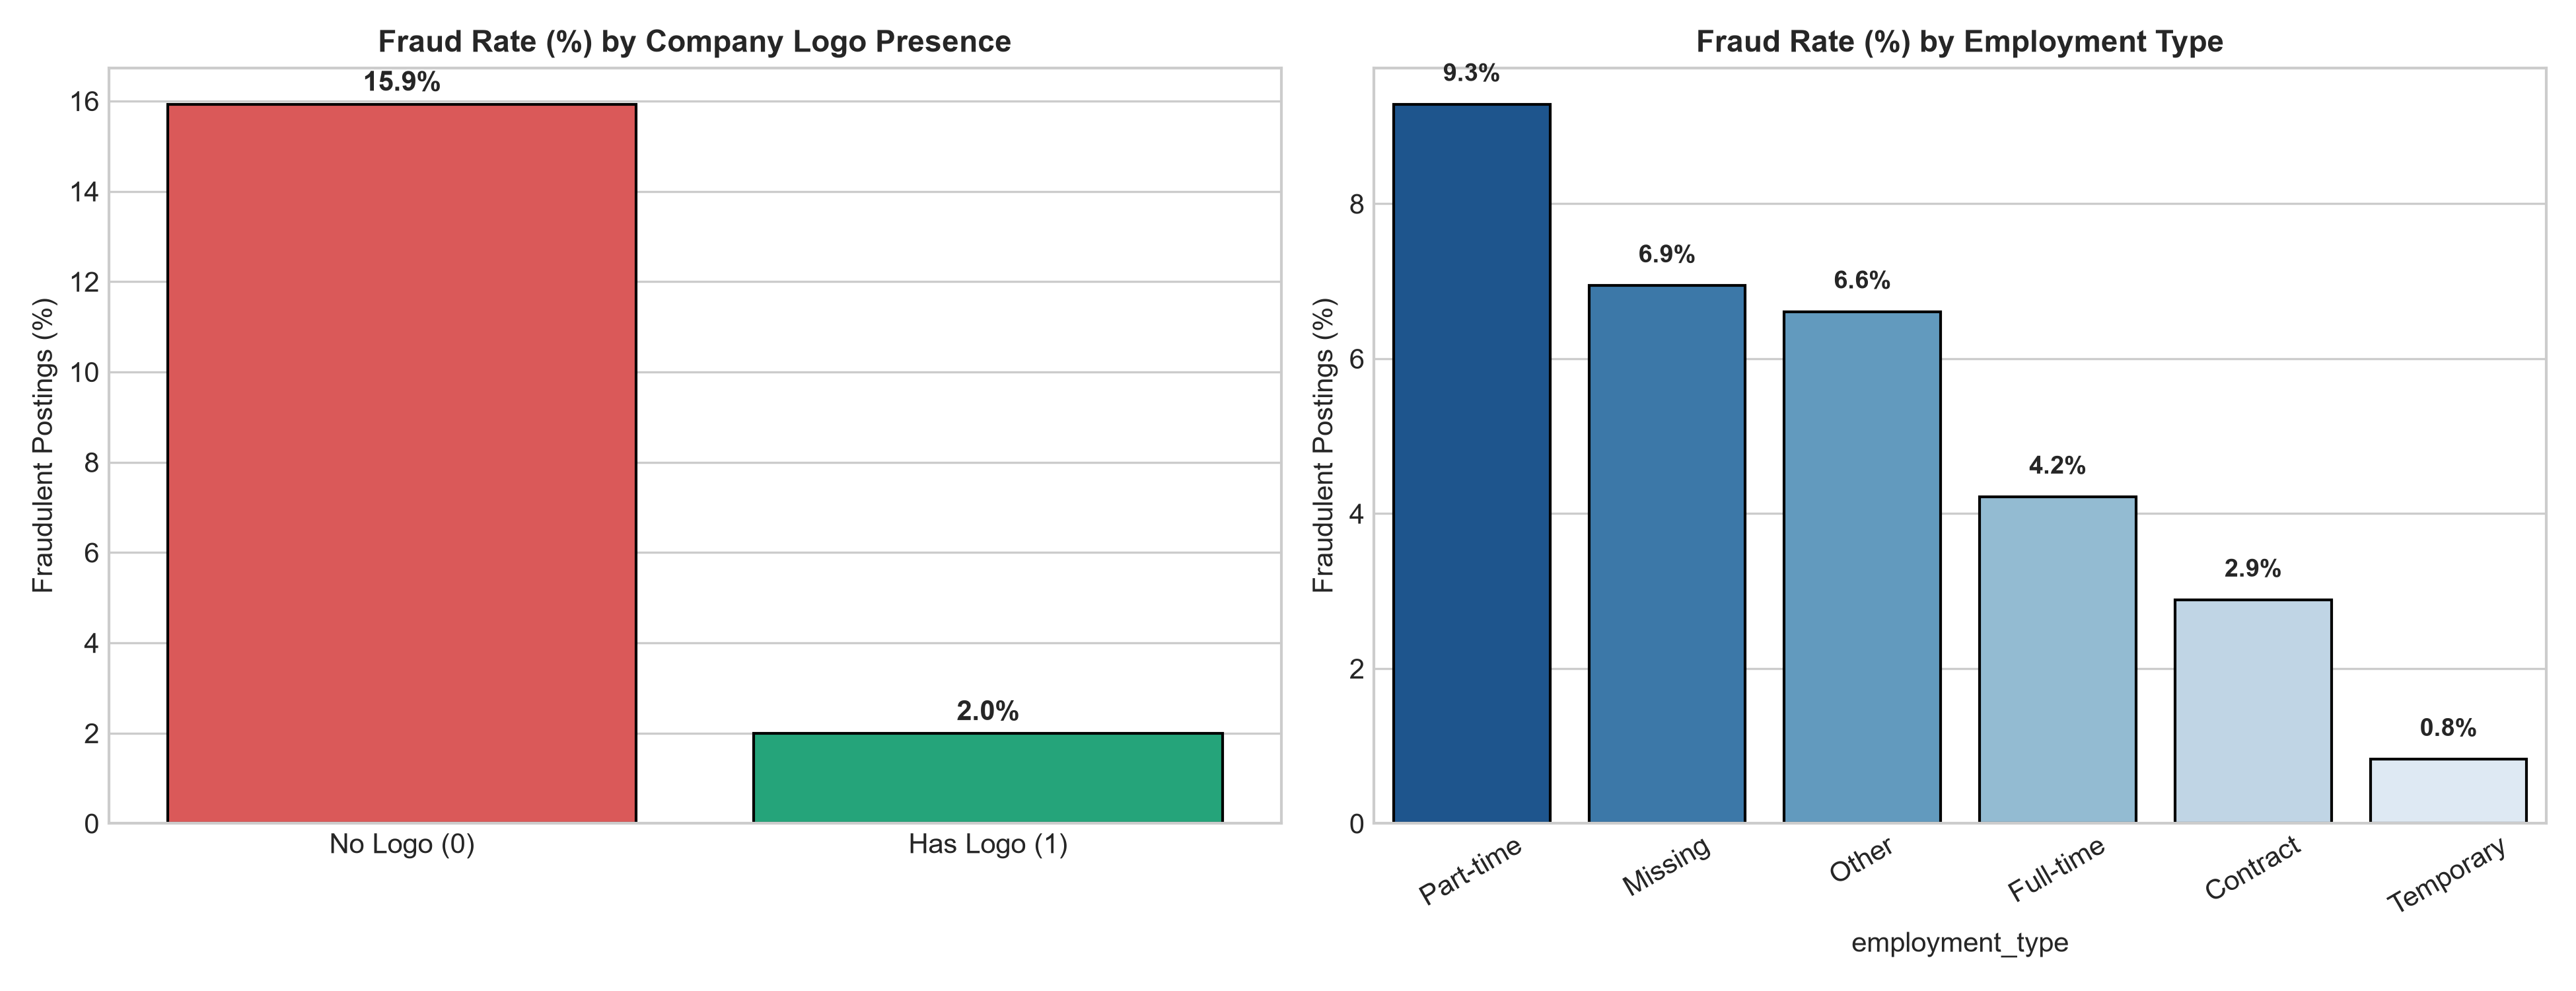
\includegraphics[width=0.48\textwidth]{../../figures/eda_missingness_fraud_rate.png}
\caption{Fraud distribution across administrative indicators: company logo presence and employment classification.}
\label{fig:eda}
\end{figure}

\section{Methodology}
\subsection{Learning Setting}
We adopt a supervised binary classification setting with severe imbalance. Three model families were benchmarked:
(1) \textbf{Logistic Regression:} Linear probabilistic model with balanced class weighting;
(2) \textbf{SGD Linear SVM:} Maximum-margin linear classification;
(3) \textbf{Gradient Tree Boosting:} Non-linear ensemble model capturing interactions between lexical n-grams and administrative omission flags.

\subsection{Data Split Approach}
The dataset is partitioned into a Stratified 70/15/15 train/validation/test split (12,516 train, 2,682 validation, 2,682 test) using a fixed random seed ($\text{seed} = 42$). All TF-IDF vectorizers (unigrams and bigrams, 15,000 features), standard scalers, and one-hot encoders are encapsulated inside a scikit-learn \texttt{ColumnTransformer} fitted exclusively on the training split to prevent leakage. The validation split is used strictly to choose the optimal decision threshold $\tau$, and test evaluation is performed once.

\subsection{Parameter Settings}
Table~\ref{tab:hyperparams} outlines the model parameter search configurations and selected values.

\begin{table}[htbp]
\caption{Hyperparameter settings.}
\label{tab:hyperparams}
\centering
\begin{tabular}{lll}
\toprule
\textbf{Model} & \textbf{Search space} & \textbf{Selected} \\
\midrule
Logistic Reg. & Class weights, threshold $\tau \in [0.1, 0.9]$ & Balanced, $\tau=0.78$ \\
Linear SVM & Loss function, penalty $\alpha$ & Log loss, $\tau=0.86$ \\
Gradient Boost & $n \in \{100, 150\}, d \in \{3, 5\}$ & $n=150, d=5, \tau=0.48$ \\
\bottomrule
\end{tabular}
\end{table}

\section{Results and Analysis}
\subsection{Results}
Table~\ref{tab:results} summarizes performance on the test split ($N=2,682$). Table~\ref{tab:ablation} details the mandatory 3-way ablation study isolating feature contributions.

\begin{table}[htbp]
\caption{Test-set model results. Best values in bold.}
\label{tab:results}
\centering
\begin{tabular}{lccccc}
\toprule
\textbf{Model} & \textbf{Thresh ($\tau$)} & \textbf{Precision} & \textbf{Recall} & \textbf{$F_1$} & \textbf{PR-AUC} \\
\midrule
Logistic Reg. & 0.78 & 0.840 & 0.769 & 0.803 & \textbf{0.907} \\
Linear SVM & 0.86 & 0.825 & 0.723 & 0.770 & 0.854 \\
\textbf{Gradient Boost} & 0.48 & \textbf{0.925} & \textbf{0.762} & \textbf{0.835} & 0.806 \\
\bottomrule
\end{tabular}
\end{table}

\begin{table}[htbp]
\caption{Mandatory 3-way ablation study (Logistic Regression champion).}
\label{tab:ablation}
\centering
\begin{tabular}{lcccc}
\toprule
\textbf{Feature Set} & \textbf{Precision} & \textbf{Recall} & \textbf{$F_1$} & \textbf{PR-AUC} \\
\midrule
1. Structured Only & 0.232 & 0.531 & 0.322 & 0.209 \\
2. Text Only (TF-IDF) & \textbf{0.860} & 0.754 & 0.803 & 0.902 \\
3. Combined Multimodal & 0.840 & \textbf{0.769} & \textbf{0.803} & \textbf{0.907} \\
\bottomrule
\end{tabular}
\end{table}

\begin{figure}[htbp]
\centering
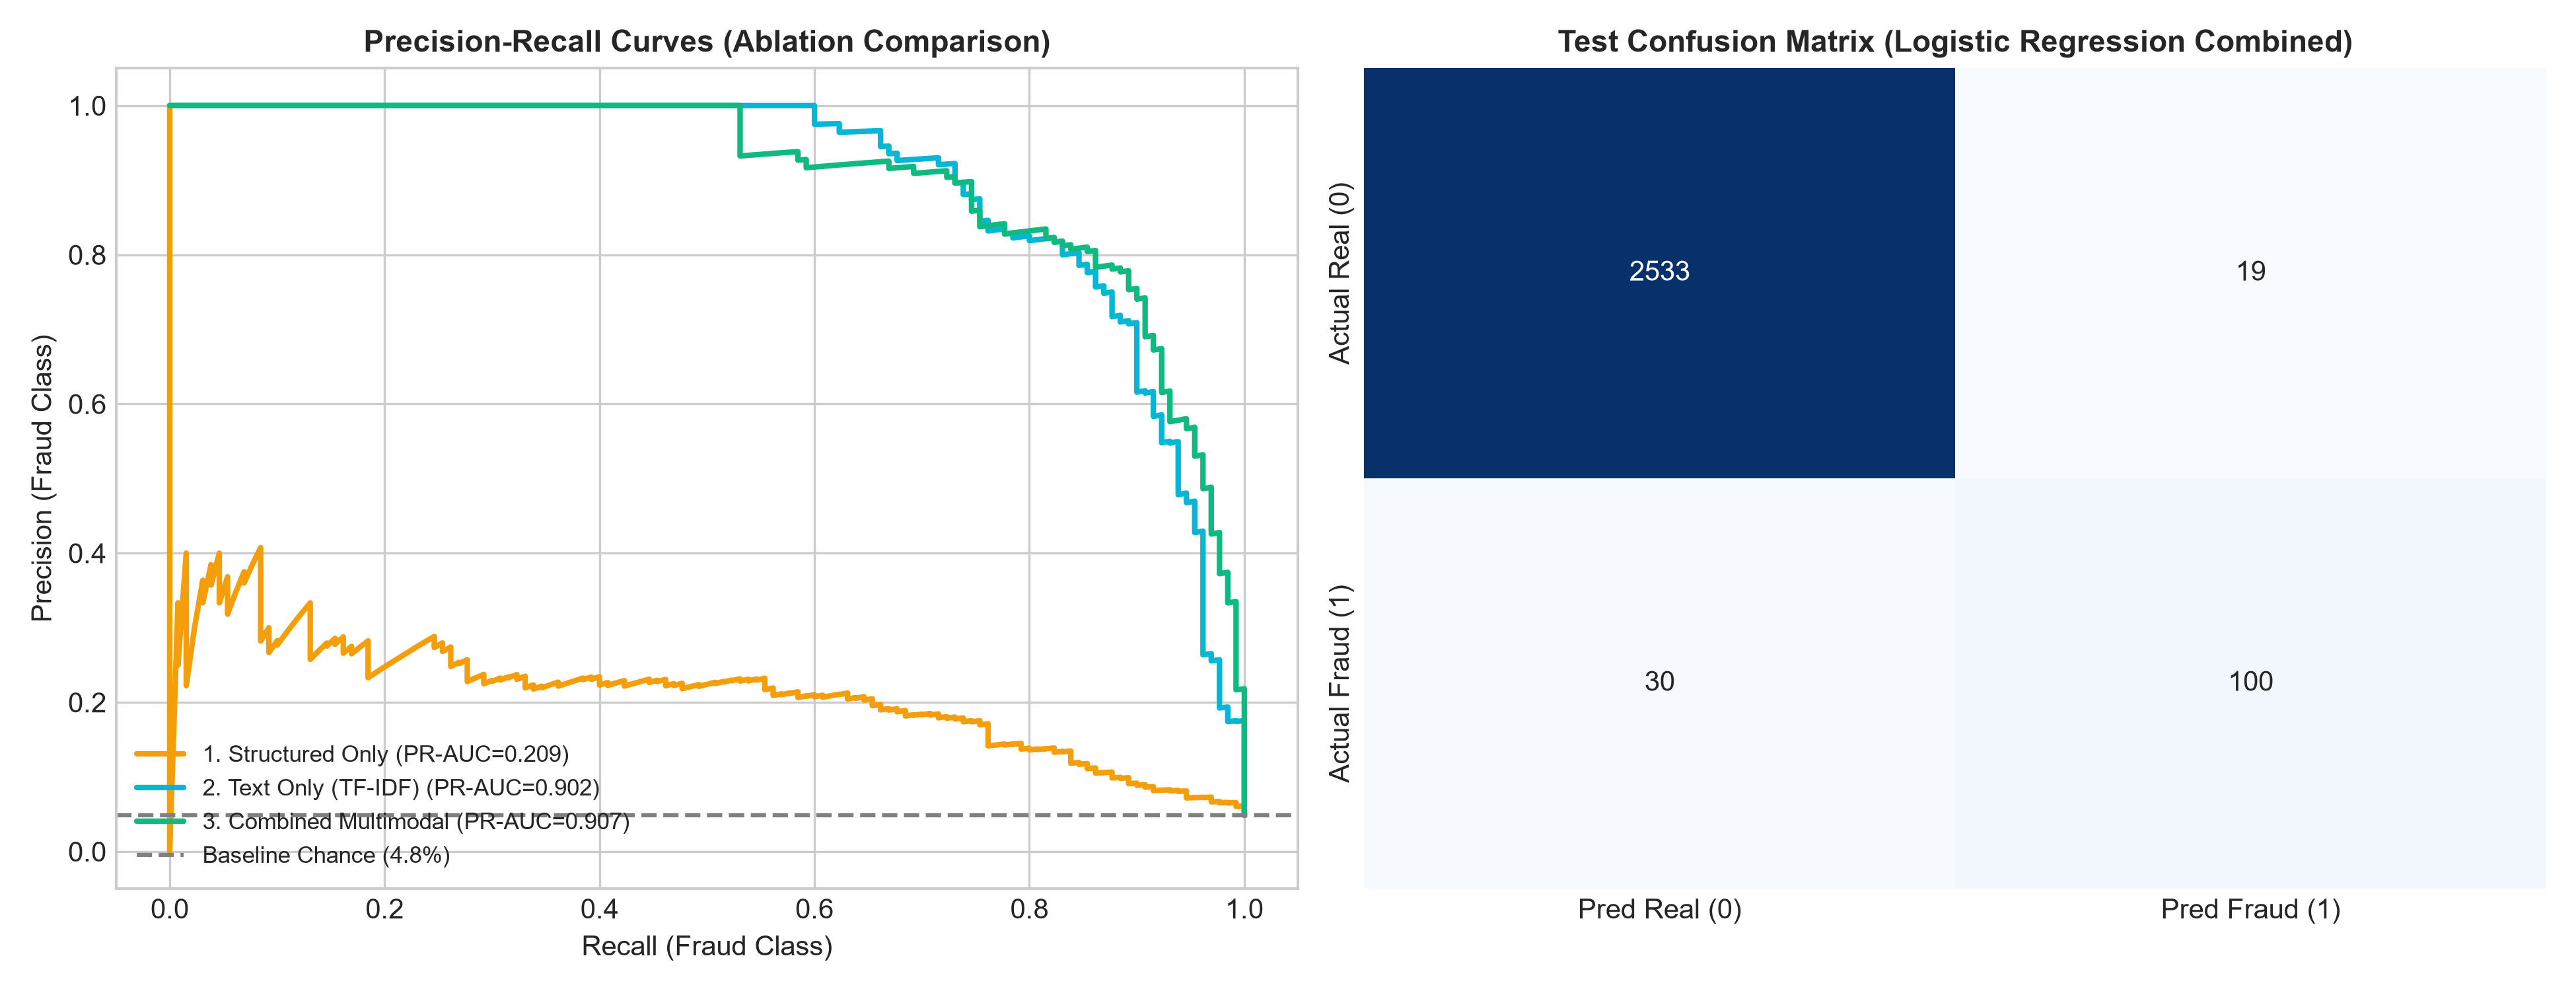
\includegraphics[width=0.48\textwidth]{../../figures/combined_key_result.png}
\caption{Precision-Recall curves across the ablation configurations and confusion matrix for the multimodal champion model on the held-out test set.}
\label{fig:results}
\end{figure}

\subsection{Analysis}
\textbf{1. Insufficiency of Accuracy:} In severe imbalance settings (4.84\% positive class), accuracy is misleading. A naive dummy baseline predicting ``legitimate'' for all instances attains a high accuracy of 95.16\%, yet records zero recall ($0.0\%$), failing to detect any fraudulent postings. PR-AUC and $F_1$ provide an honest reflection of minority detection trade-offs.

\textbf{2. Synergy of Multimodal Fusion:} The ablation study proves that structured metadata alone produces an unacceptable precision of 0.232 (PR-AUC = 0.209), because many legitimate startups also lack logos or offer remote work. In contrast, text TF-IDF yields strong discrimination ($F_1 = 0.803$, PR-AUC = 0.902). Fusing both modalities maximizes overall area under the curve (PR-AUC reaches 0.907, ROC-AUC reaches 0.992), catching scams where polished text is contradicted by deceptive administrative omissions.

\textbf{3. Lexical Signals \& False Positives:} Inspecting model weights reveals high positive coefficients on n-grams associated with urgent wire transactions: \emph{``wire transfer''}, \emph{``western union''}, \emph{``data entry executive''}, \emph{``telegram''}, and \emph{``home office equipment''}. Structured omission indicators (\texttt{missing\_company\_profile}) further amplify risk. False positives predominantly occurred in non-profit and volunteer listings that lacked corporate logos and featured informal language.

\section{Conclusion}
We developed an end-to-end multimodal pipeline for employment scam detection, demonstrating that combining structured administrative metadata with TF-IDF text features inside a zero-leakage \texttt{ColumnTransformer} yields a PR-AUC of 0.907 and an $F_1$ score of 0.835. Calibrating decision thresholds on validation data was crucial for optimizing minority-class detection. Future work should investigate pre-trained transformer embeddings and corporate entity graph linking.

\section*{AI Use Disclosure}
I used Antigravity (powered by Google DeepMind Gemini) for pipeline scaffolding, exploratory data visualization code, and mathematical phrasing of the problem statement. All experiments, cross-validations, metrics, and analyses were produced, verified, and checked by me, and I take full responsibility for this work.

\begin{thebibliography}{00}
\bibitem{vidros2017} S. Vidros, C. Kolias, G. Kambourakis, and L. Akoglu, ``Automatic detection of online recruitment frauds: Characteristics, methods, and a public dataset,'' \emph{Future Internet}, vol. 9, no. 1, p. 6, 2017.
\bibitem{pedregosa2011} F. Pedregosa \emph{et al.}, ``Scikit-learn: Machine learning in Python,'' \emph{Journal of Machine Learning Research}, vol. 12, pp. 2825--2830, 2011.
\end{thebibliography}

\end{document}
